\documentclass{article}
\usepackage{packages}
\usepackage[utf8]{inputenc}
\usepackage[T1]{fontenc}
\usetikzlibrary{shapes.geometric}

\begin{document}

\section{Electrons I (FEG)}

\subsubsection*{(a)}
For a system at temperature $T$ the free energy is given by 
\begin{equation*}
    G(p, T) = E + pV - TS
    \label{eq:FreeEneergy}
\end{equation*}
where the pressure $p$, the volume $V$ and the temperature $T$ are connected through a state equation of the type $\phi(p, V, T) = 0$ that depends
on the system. \\
For $T=0$ equation \ref{eq:FreeEneergy} reduces to
\begin{equation}
    G(p, T) = E + pV
\end{equation}
where $E$ is the energy of the system. \\
In the Free Fermi Electron Gas model the energy can be computed as
\begin{equation}
    E(T) = \int_{E_{min}}^{E_{max}} d\epsilon \ DOS(\epsilon) \ f_{FD}(\epsilon, T) \ \epsilon 
\end{equation}
where $f_{FD}(\epsilon)$ is the Fermi-Dirac distribution 
\begin{equation*}
    f_{FD}(\epsilon) = \frac{1}{e^{(\epsilon_i - \mu)/k_B T} + 1}
\end{equation*}
and indicates the average number of fermions in a single-particle state. \\
In the limit of zero temperature one gets
\begin{equation}
    \lim_{T \to 0} E(T) = \int_{E_{min}}^{E_{max}} d\epsilon \ \lim_{T \to 0} \ DOS(\epsilon) \ f_{FD}(\epsilon, T) \ \epsilon
    \label{eq:energy_FEFG}
\end{equation}
The 3D density of states function 
\begin{equation}
    DOS(\epsilon) = \frac{V}{2\pi^2} \ \left(\frac{2m}{\hbar^2}\right)^{3/2} \ \epsilon^{1/2}
\end{equation}
does not depend on the temperature, while the Fermi-Dirac distribution function in the limit $T \to 0$ reduces to 
\begin{equation}
    \lim_{T \to 0} f_{FD}(\epsilon) = 
    \begin{cases}
        1 \qquad \text{if } \epsilon < \mu \\
        \frac{1}{2} \qquad \text{if } \epsilon = \mu \\ 
        0 \qquad \text{if } \epsilon > \mu
    \end{cases}
\end{equation}
so that \ref{eq:energy_FEFG} becomes 
\begin{equation*}
    E \equiv E(T=0) = \frac{V}{2\pi^2} \ \left(\frac{2m}{\hbar^2}\right)^{3/2} \int_{E_{min}}^{E_{max}} \epsilon^{3/2} \, d\epsilon
\end{equation*}
In the last integral the extrema are $E_{min} = 0$ and $E_{max} = \epsilon_F$,. $E_F$ is the Fermi energy which is, by definition, the energy of 
the last occupied state. Hence
\begin{equation}
    E = \frac{V}{5\pi^2} \ \left(\frac{2m}{\hbar^2}\right)^{3/2} \, \epsilon_F^{5/2}
    \label{eq:energy_energyfermi}
\end{equation}
and using the relation 
\begin{equation*}
    \epsilon_F = \frac{\hbar^2}{2m} \left(\frac{3\pi^2N}{V}\right)^{1/3}
\end{equation*}
one obtains
\begin{equation*}
    E = \frac{V}{5\pi^2} \ \left(\frac{2m}{\hbar^2}\right)^{3/2} \, \epsilon_F^{5/2}
\end{equation*}
The pressure can then be calculated by the Maxwell relation 
$$p = -\frac{\partial E}{\partial V} = \frac{2}{3} \ \frac{1}{5\pi^2 V^{2/3}} \ \frac{\hbar^2}{2m} (3\pi^2N)^{5/3} = \frac{2}{3}\frac{E}{V}$$
so that 
$$G = E + pV = \frac{5}{3} E = \frac{2}{3} \frac{V}{5\pi^2} \ \left(\frac{2m}{\hbar^2}\right)^{3/2} \ \epsilon^{5/2}$$
which can be rearranged as
$$G = N \epsilon_F$$
Equating this result to the formula given in the text of the exercise $G = N\mu$ one concludes that at temperature $T=0$ 
\begin{equation}
    \epsilon_F = \mu
\end{equation}

\subsubsection*{(b)}
By looking at figure \ref{fig:fFD_mu}, one can notice that for $T=0.01 \, T_F$ and $T=0.1 \, T_F$ (blue and green lines) the dashed curves overlap with the continuous lines. This means that the approximation 
$\mu = \epsilon_F$ in the Fermi-Dirac distribution is legitimate. On the other side for $T=T_F/2$ one can see that the dashed line does not overlap with the continous one and in particular the maximum difference 
occurs at $\epsilon = \epsilon_F$, where the approximated function ($\mu = \epsilon_F$) is always $1/2$ and the true function is not. This means that the approximation is not anymore valid.
\begin{figure}[htp]
    \centering 
    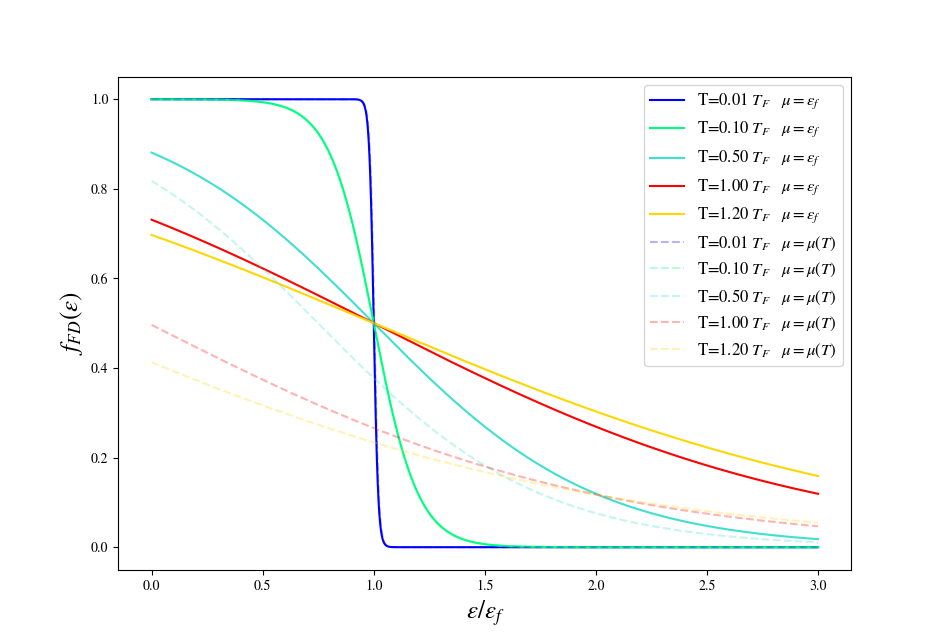
\includegraphics[scale=0.5]{scripts/f_fd_mu.png}
    \caption{Fermi-Dirac distribution for various temperature values. The continous lines correspond to 
    the distribution drawn by keeping the chemical potential constant at $\mu=_{epsilon_F}$, while the dashed lines represent the true relations.}
    \label{fig:fFD_mu}
\end{figure}

\subsubsection*{(c)}
The number of orbitals whose energy is less than or equal to $\epsilon$ is given by 
\begin{equation}
    N = \frac{V}{3\pi^2} \left(\frac{2m\epsilon}{\hbar^2}\right)^{3/2}
    \label{eq:N_orbitals}
\end{equation}
At $T=0$ all the electrons lie in the lowest-energy orbitals and the Fermi energy $\epsilon_F$
corresponds to the energy of the last filled orbital. Hence in this particular case equation \ref{eq:N_orbitals}
gives exactly the number of electrons divided by 2 (there are 2 electrons for each orbital). By indicating with $n$ the number of electrons,
one has that 
\begin{equation}
    n = 2\frac{V}{3\pi^2} \left(\frac{2m\epsilon_F}{\hbar^2}\right)^{3/2}
    \label{eq:n_elect1}
\end{equation}
but on the other side
\begin{equation*}
    n = \int_0^{+\infty} \, 2DOS(\epsilon) \, f_{FD}(\epsilon) \, d\epsilon
    \label{eq:n_elect2}
\end{equation*}
One can now impose the equality between \ref{eq:n_elect1} and \ref{eq:n_elect2}: in particular expression \ref{eq:n_elect2} is a function of the chemical potential $\mu$ and the temperature $T$ and 
the equation can be written as 
\begin{equation*}
    N_0 = g(\mu, T)
\end{equation*}
where $N_0$ is given by \ref{eq:n_elect1} and $g(\mu, T)$. \\
The equation can be solved numerically using the following procedure:
\begin{enumerate}
    \item Fix a value for the temperature $T_1$
    \item The equation is now an equation in one variable $\mu$ an can be solved via traditional numerical methods to obtain a corresponding value $\mu_1$.
    \item Store the values $(T_1, \mu_1)$
    \item Select a value $T_1$ and repeat from point $1)$
\end{enumerate}
In this way we obtain multiple couples $(T_i, \mu_i)$ that can be plotted to give a graphical representation of the function $\mu(T)$ (see figure \ref{fig:chemical_potential})
\begin{figure}[hbtp]
    \centering 
    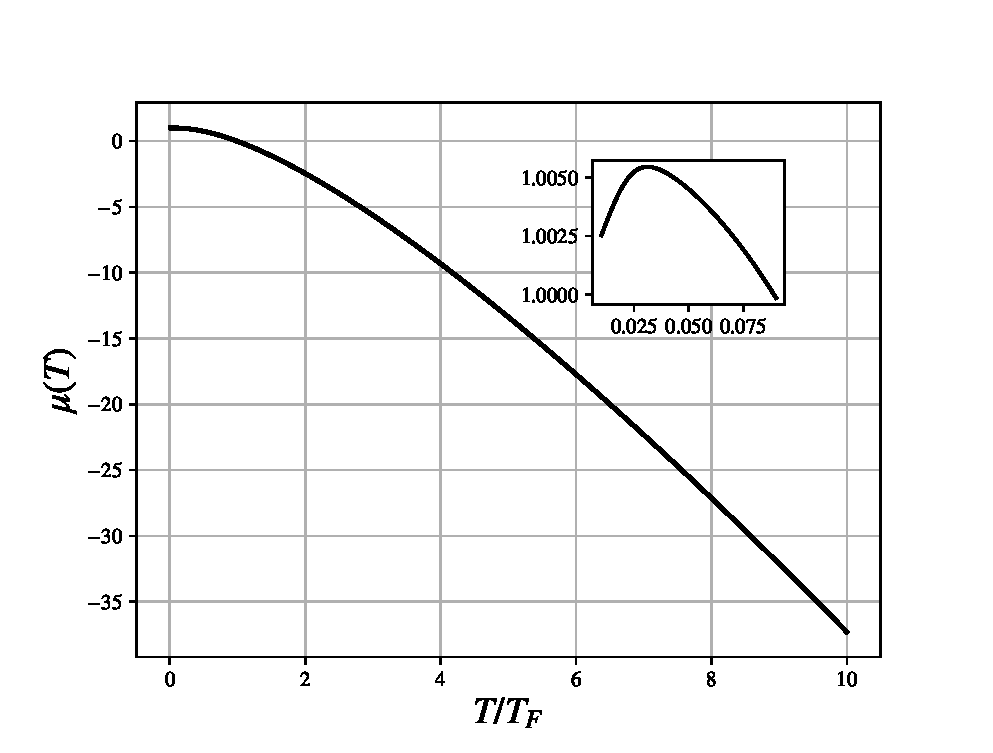
\includegraphics[scale=0.7]{scripts/mu_T.eps}
    \caption{Chemical potential as a function of temperature. The small window on top right is a zoom on the low-temperature area. It shows that for low temperature
    the chemical potential dependence on the temperature can be well approximated by a parabola of the type $\mu(T) = \mu(T=0) - \alpha T^2 = \epsilon_F - \alpha T^2$}
    \label{fig:chemical_potential}
\end{figure}

\subsubsection*{(d)}
The curves are already reported in figure \ref{fig:fFD_mu} as dashed lines, but I report them here alone for clarity
\begin{figure}
    \centering
    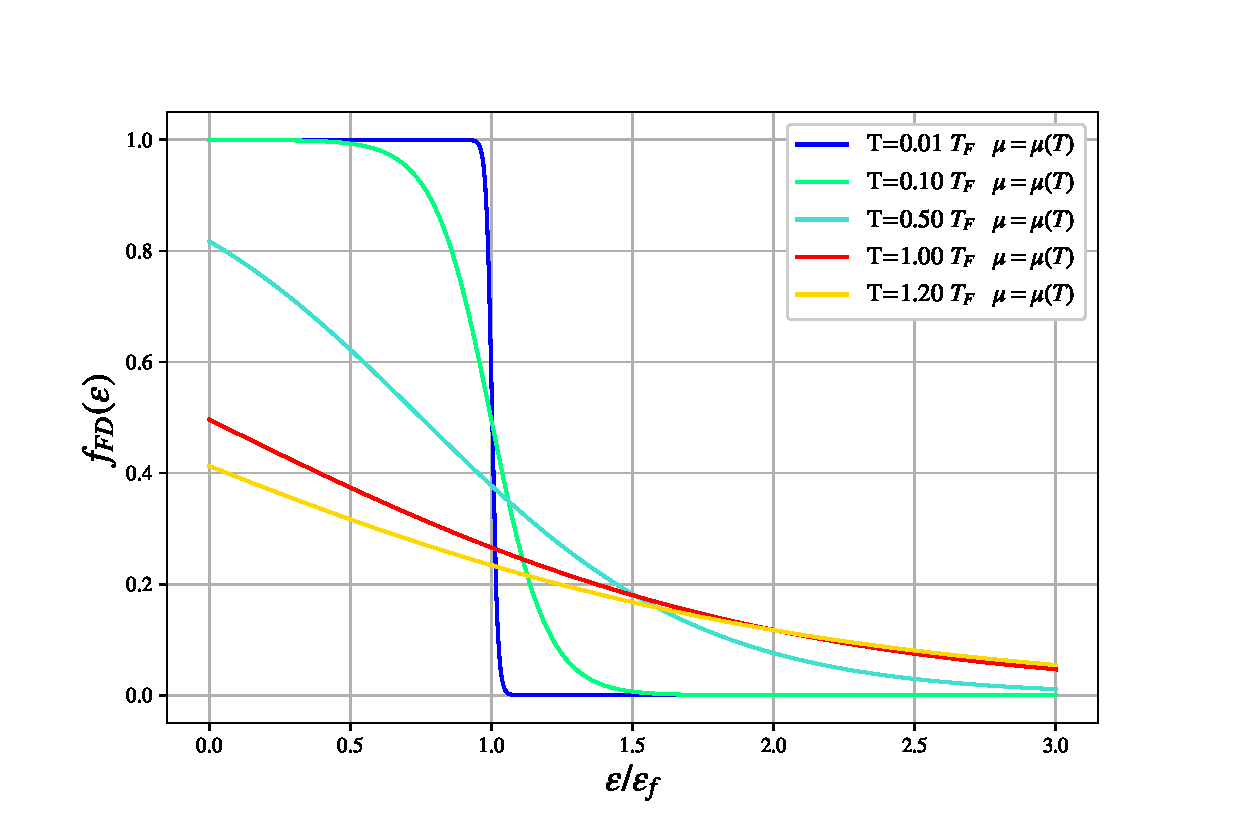
\includegraphics[scale=0.5]{scripts/f_fd_mu_T.eps}
    \caption{Fermi-Dirac distribution for various value of temperature. The depence of the chemical $\mu$ on the temperature is taken into account.}
    \label{fig:fFD_mu_T}
\end{figure}

\subsubsection*{(e)}
The energy of the system can be computed as 
\begin{equation*}
    E = \int_0^{+\infty} DOS(\epsilon) \, f_{FD}(\epsilon, T) \, \epsilon \, d\epsilon
\end{equation*}
The electrons' heat capacity contribution is
\begin{equation*}
    C = \frac{dE}{dT} = \int_0^{+\infty} DOS(\epsilon) \, \frac{\partial f_{FD}(\epsilon, T)}{\partial T} \, \epsilon \, d\epsilon
\end{equation*}
Since the number of electrons is independent of the temperature the last expression is equivalent to 
\begin{equation*}
    C = \frac{dE}{dT} - \epsilon_F\frac{dN}{dT} = \int_0^{+\infty} DOS(\epsilon) \, \frac{\partial f_{FD}(\epsilon, T)}{\partial T} \, (\epsilon -\epsilon_F) \, d\epsilon
\end{equation*}
Let us now consider the quantum limit $k_BT \ll \epsilon_F$: it can be easilly seen from figure (REFFF) that $\frac{df_{FD}}{d\epsilon}$ is significantly different from zero only 
in a small region of width $2k_BT$ centered in $\epsilon=\epsilon_F$. Hence
\begin{equation*}
    C \approx DOS(\epsilon_F) \int_0^{+\infty} \frac{\partial f_{FD}(\epsilon, T)}{\partial T} \, (\epsilon - \epsilon_F) \, d\epsilon = 
    DOS(\epsilon_F) k_B^2T \int_{-\epsilon_F/k_BT}^{+\infty} \frac{e^x}{(e^x + 1)^2} \, dx 
\end{equation*}
where I made the change of variable $x=(\epsilon - \epsilon_F)/k_BT$ and I used the fact that 
\begin{equation*}
    \frac{\partial f_{FD}(\epsilon, T)}{\partial T} = \frac{\epsilon - \epsilon_F}{k_BT^2} \frac{exp((\epsilon - \epsilon_F)/k_BT)}{[exp((\epsilon - \epsilon_F)/k_BT) + 1]^2}
\end{equation*}
that is I used the approximation $\mu \approx \epsilon_F$ (valid for the low temperature range).
Since we assumed $k_BT \ll \epsilon_F$ the lower extrema can be approximated to $-\infty$. The integral is now a known integral and the value is $\pi^2/3$. Using the fact that 
$DOS(\epsilon_F) = \frac{3N}{2\epsilon_F}$ the estimated specific heat is 
\begin{equation*}
    C \approx \frac{\pi^2}{2} N k_B^2 \frac{T}{E_F} = \frac{\pi^2}{2} N k_B \frac{T}{T_F}
\end{equation*}

\section{Exercise II}
Let us first consider a simple delta potential $V(x) = V_0 \, \delta(x)$ and the Schroedinger equation 
\begin{equation*}
    -\frac{\hbar^2}{2m}\psi''(x) + V(x) \psi(x) = E \psi(x)
\end{equation*}
Let us integrate both members between $-\epsilon$ and $+\epsilon$ and let $\epsilon \to 0$, we obtain 
\begin{equation*}
    \lim_{\epsilon \to 0} -\frac{\hbar^2}{2m} \left(\psi'(\epsilon) - \psi'(-\epsilon)\right) + V_0\int_{-\epsilon}^{+\epsilon} \delta(x) \psi(x) = \lim_{\epsilon \to 0} 2\epsilon E \psi(0)
\end{equation*} 
or 
\begin{equation*}
    \psi'(0^+) - \psi'(0^-) = \frac{2mV_0}{\hbar^2}\psi(0)
\end{equation*}
This equation can be read as a condition on the discontinuity of the derivative of the function $\psi(x)$ across the $\delta$. \\
Now let us return to the Dirac delta comb potential $V(x) = \sum_{n=-\infty}^{+\infty} \delta(x+na)$. The potential is clearly periodic with period $a$. Hence
one can make use of the Bloch's theorem which states that the wavefunctions satisfy the conditions
\begin{equation*}
    \psi(x) = e^{iQx} u(x)
\end{equation*}
where $Q=\frac{2\pi}{na}$ and $u(x)$ satisfies in turn
\begin{equation*}
    u(x+na) = u(x)
\end{equation*}
One can now restrict the domain to $0<x<a$ and solve the problem in this interval, imposing then the Bloch condition to obtain the solution 
to the complete theorem. For $0<x<a$ the solution is a combination of plane waves
\begin{equation*}
    \psi(x) = Ae^{ikx} + Be^{-ikx}
\end{equation*}
By using the Bloch's theorem one can relate the solution for $a<x<2a$ to the one for $0<x<a$
\begin{equation*}
    \frac{\psi(x)}{\psi(x+a)} = \frac{u(x)e^{iQx}}{u(x+a)e^{iQx}e^{iqa}} = e^{-iQa}
\end{equation*}
So that 
$\psi(x+a) = e^{iQa} \, \psi(x)$
Let us now impose the continuity of $\psi(x)$ and the discontinuity of $\psi'(x)$ on the edge between the two zones at $x=a$
$$\begin{cases}
    eq1
\end{cases}$$
which can be reduced
\begin{equation*}
    \cos(Qa) = \cos(ka) + \frac{V_0}{2ka} \sin(ka)
\end{equation*}
The admitted values of $k$ for the system are those that satisfy the above equation. The corresponding energies are then $E_k = \frac{\hbar^2k^2}{2m}$.
The last equation has solution only if $|cos(ka) + \frac{V_0}{2ka} \sin(ka)| < 1$. 
For $|cos(ka) + \frac{V_0}{2ka} \sin(ka)| > 1$ there are no solutions: this means that therethose $k-$vectors are admitted by the system, hence those energies are not admitted.


\section*{Exercise 3}

\subsubsection*{(a)}
One possible way describe a disordered material is by mean of a two-level system. According to this model there are single atoms or group of atoms in the material that can lie in one of two adiacent minima of 
a potential and can quantum tunnel between the states. In this sense each of these atoms (or aggregate of atoms) can be seen as a two-level system. The energy of the whole system is then the sum of the energies of each two-level system (TLS). \\
Let us label the minima $1$ and $2$ with related energies $E_1=0$ and $E_2=\epsilon$. \\
Each TLS can be described as a member of a canonical ensemble whose partition function is $Z = e^{-\beta E_1} + e^{-\beta E_2} = 1 + e^{-\beta \epsilon}$ where $\beta = 1/k_BT$. According to this, the probabilities for each TLS to be in one of the two levels are
\begin{equation*}
    p_1 \equiv p(E_1) = \frac{e^{-\beta E_1}}{Z} = \frac{1}{1 + e^{-\beta \epsilon}} \qquad p_2 \equiv p(E_2) = \frac{e^{-\beta E_1}}{Z} = \frac{e^{-\beta \epsilon}}{1 + e^{-\beta \epsilon}}
\end{equation*}
The average energy for each TLS is now
\begin{equation*}
    E_{TLS} \equiv \langle E_{TLS}(\epsilon) \rangle = p_1 E_1 + p_2 E_2 = \frac{\epsilon e^{-\beta\epsilon}}{1 + e^{-\beta\epsilon}} = \frac{\epsilon}{1 + e^{\beta\epsilon}}
\end{equation*}
And each TLS has an average heat capacity of
\begin{equation*}
    c_v = \frac{\partial E}{\partial T} = k_B \beta^2 \epsilon^2 \frac{e^{\beta \epsilon}}{(e^{\beta \epsilon} + 1)^2}
\end{equation*}
Now, in the material, there might be more that one TLS with the same energy: let us call $DOS(\epsilon)$  the number of states with energy $\epsilon$ (density of states). According to this definition the total energy of the system is given by 
\begin{equation*}
    E = \int_0^{+\infty} DOS(\epsilon) \ E_{TLS}(\epsilon) \ d\epsilon = k_B \int_0^{+\infty} DOS(\epsilon) \ \frac{\epsilon^2\beta^2 e^{\beta\epsilon}}{(e^{\beta \epsilon}+1)^2} \ d\epsilon
\end{equation*}
And the heat capacity of the material is 
\begin{equation}
    C = \frac{\partial E}{\partial T} = \int_0^{+\infty} DOS(\epsilon) \ \frac{\partial E_{TLS}(\epsilon)}{\partial T} \ d\epsilon
    \label{eq:heat_capacity}
\end{equation}
The exercise provides a model with a time dependent density of states that is
\begin{equation}
    DOS(\epsilon, t) = \frac{P_0}{2}\log\left(\frac{4t}{\tau(\epsilon)}\right)
    \label{eq:DOS_t_dep}
\end{equation}
where
\begin{equation}
    \frac{1}{\tau(\epsilon)} = K \, \epsilon^3 \coth\left(\frac{\beta\epsilon}{2}\right)
    \label{eq:tau_eps}
\end{equation}
By inserting \ref{eq:tau_eps} into \ref{eq:heat_capacity} one obtains
\begin{equation}
    C = \frac{k_BP_0}{2} \ \int_0^{+\infty} \log\left(\frac{4t}{\tau(\epsilon)}\right) \ \frac{\beta^2\epsilon^2 e^{\beta\epsilon}}{(e^{\beta \epsilon} + 1)^2}
    \label{eq:big_integral}
\end{equation}
The integral cannot be solved analytically but it can be approximated as explained in the following lines. \\
The function $E_{TLS}(\epsilon) = \beta^2\epsilon^2e^{\beta\epsilon}/(e^{\beta\epsilon} + 1)^2$ is peaked at the point
$\epsilon \approx 2.5/\beta = 2.5 \, k_B T$ and the peak becomes more narrow as the temperature decreases (or $\beta$ increases). This means that the integrand is significantly far from zero only 
in a narrow region around $\epsilon_0 \approx 2.5 k_B T$. Let us call $\epsilon_{min}$ and $\epsilon_{max}$ the two extrema of the peak area (see figure \ref{fig:peak} on the left). In this region the other term in the integral $DOS(\epsilon) = \log(4t/\tau(\epsilon))$
is practically constant as can be seen in figure \ref{fig:peak} on the right. 
\begin{figure}[htp]
\centering
\begin{minipage}{0.4\textwidth}
    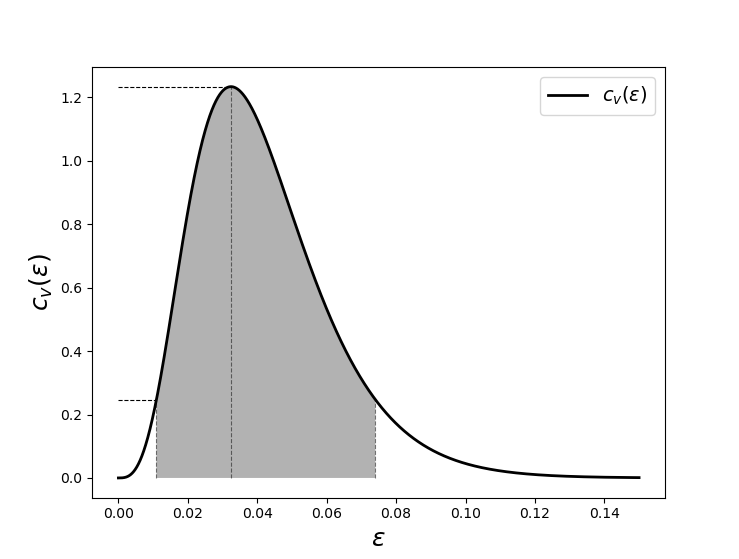
\includegraphics[scale=0.45]{scripts/cv_eps.png}
\end{minipage}
\hfill
\begin{minipage}{0.45\textwidth}
    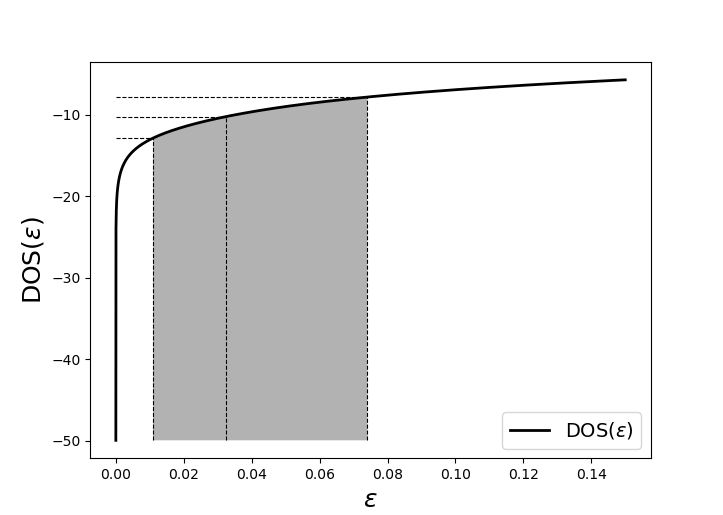
\includegraphics[scale=0.45]{scripts/DOS_eps.png}
\end{minipage}
\caption{The energy of the system is the integral of the product of the plotted functions. Since the left one goes rapidly to zero
outside the grey area, the integral can be well approximated considering the contributions of the grey area only. In this range the other function (on the right) varies
slowly and can be indeed approximated by a constant value.}
\label{fig:peak}
\end{figure}
This means that one can approximate it with the value in the $\epsilon_0$, that is
\begin{equation*}
    DOS(\epsilon, t) = \log(4t/\tau(\epsilon)) \approx \log(4t/\tau(\epsilon_0)) \qquad \text{for} \quad \epsilon \in [\epsilon_{min}, \epsilon_{max}]
\end{equation*}
Equation \ref{eq:big_integral} becomes then 
\begin{equation}
    C \approx \frac{k_BP_0}{2} \log(4t/\tau(\epsilon_0)) \ \int_0^{+\infty} \beta^2\epsilon^2 \frac{e^{\beta\epsilon}}{(e^{\beta\epsilon}+1)^2} \, d\epsilon =
    A \log(4t/\tau(\epsilon_0))
\end{equation}
where 
\begin{equation*}
    A = \frac{k_BP_0}{2} \int_0^{+\infty} \beta^2\epsilon^2 \frac{e^{\beta\epsilon}}{(e^{\beta\epsilon}+1)^2} \, d\epsilon
\end{equation*}

\subsubsection*{(b)}
Let us consider a system at temperature $T_1$ and a reservoir at temperature $T_0$. When the system is put into contact
with the reservoir the temperature of the system decreases or increases until it reaches $T_0$. One can calculate the energy difference between the two states: this can be done in two ways:
\begin{enumerate}
    \item By integrating the specific heat between the two temperatures
    \item By using the definition of average energy in a canonical ensemble
\end{enumerate}
I hereby follow the second path but it is competely equivalent to the first one. \\
One now has that
\begin{equation*}
    \Delta E = E(T_1) - E(T_0)
\end{equation*}
where 
\begin{equation*}
    E(T) = \int_0^{+\infty} DOS(\epsilon) \, E_{TLS}(\epsilon) \, d\epsilon = 
    \frac{P_0}{2}\int_0^{+\infty} \log(4t/\tau(\epsilon)) \frac{\epsilon }{e^{\beta\epsilon}+1} \, d\epsilon
\end{equation*}
The difference of the energy between the two states is either released or absorbed during the process depending on the relative temperature. The corresponding power is simply the derivative of
the energy with respect to time and it gives 
\begin{gather*}
    \dot q(t) = \frac{d \Delta E}{dt} = 
    \frac{k_BP_0}{2} \int_0^{+\infty} \frac{\partial \log(4t/\tau(\epsilon))}{\partial t} \ \left(\frac{\epsilon}{e^{\beta_1\epsilon} + 1} - \frac{\epsilon}{e^{\beta_0\epsilon} + 1} \right)\, d\epsilon = \\
    = \frac{k_BP_0}{2} \frac{1}{t} \int_0^{+\infty} \ \left(\frac{\epsilon}{e^{\beta_1\epsilon} + 1} - \frac{\epsilon}{e^{\beta_0\epsilon} + 1} \right) \, d\epsilon = \frac{B}{t} 
\end{gather*}
The constant $B$ can be computed by evaluating the integral. After a change of variable $x = \beta\epsilon$ one has that
\begin{gather*}
    \dot q(t) = \frac{P_0}{2\beta_1^2 \, t} \int_0^{+\infty} \frac{x}{e^x + 1} - \frac{P_0}{2\beta_0^2 \, t} \int_0^{+\infty} \frac{x}{e^x + 1} = \\
    = \frac{P_0\pi^2}{24t} \left(\frac{1}{\beta_1^2} - \frac{1}{\beta_0^2}\right) = 
    \frac{k_B^2P_0\pi^2}{24t} \left(T_1^2 - T_0^2\right) = \frac{B}{t}
\end{gather*} 
So that $B = \frac{k_B^2 P_0 \pi^2}{24} \, (T_1^2 - T_0^2)$
\end{document}